% Template for ICME 2018 paper; to be used with:
%          spconf.sty  - ICASSP/ICIP/ICME LaTeX style file, and
%          IEEEbib.bst - IEEE bibliography style file.
% --------------------------------------------------------------------------
\documentclass{article}
\usepackage{spconf,amsmath,epsfig}
\usepackage{graphicx}
\usepackage{subfigure}
\pagestyle{empty}


\begin{document}\sloppy

% Example definitions.
% --------------------
\def\x{{\mathbf x}}
\def\L{{\cal L}}


% Title.
% ------
\title{A Hybrid System Integrating Calibration and Registration for Accurate 3D Reconstruction}
%
% Single address.
% ---------------
\name{Zhehan Song, Xuejin Chen}
\address{University of Science and Technology of China}


\maketitle



\section{Global Camera Calibration}
The cameras in our 3D reconstruction system are placed on the periphery of the room pointing inwards, only the neighbouring cameras have overlapping fields of view. We found that if we calibrate the cameras pairwisely, accumulative error will occur and can be seen obviously in the result of the reconstruction. After the initial calibration, we optimize the extrinsic parameters globally using a checkerboard.

\subsection{Multi-camera system}
\begin{figure*}[ht]
\centering
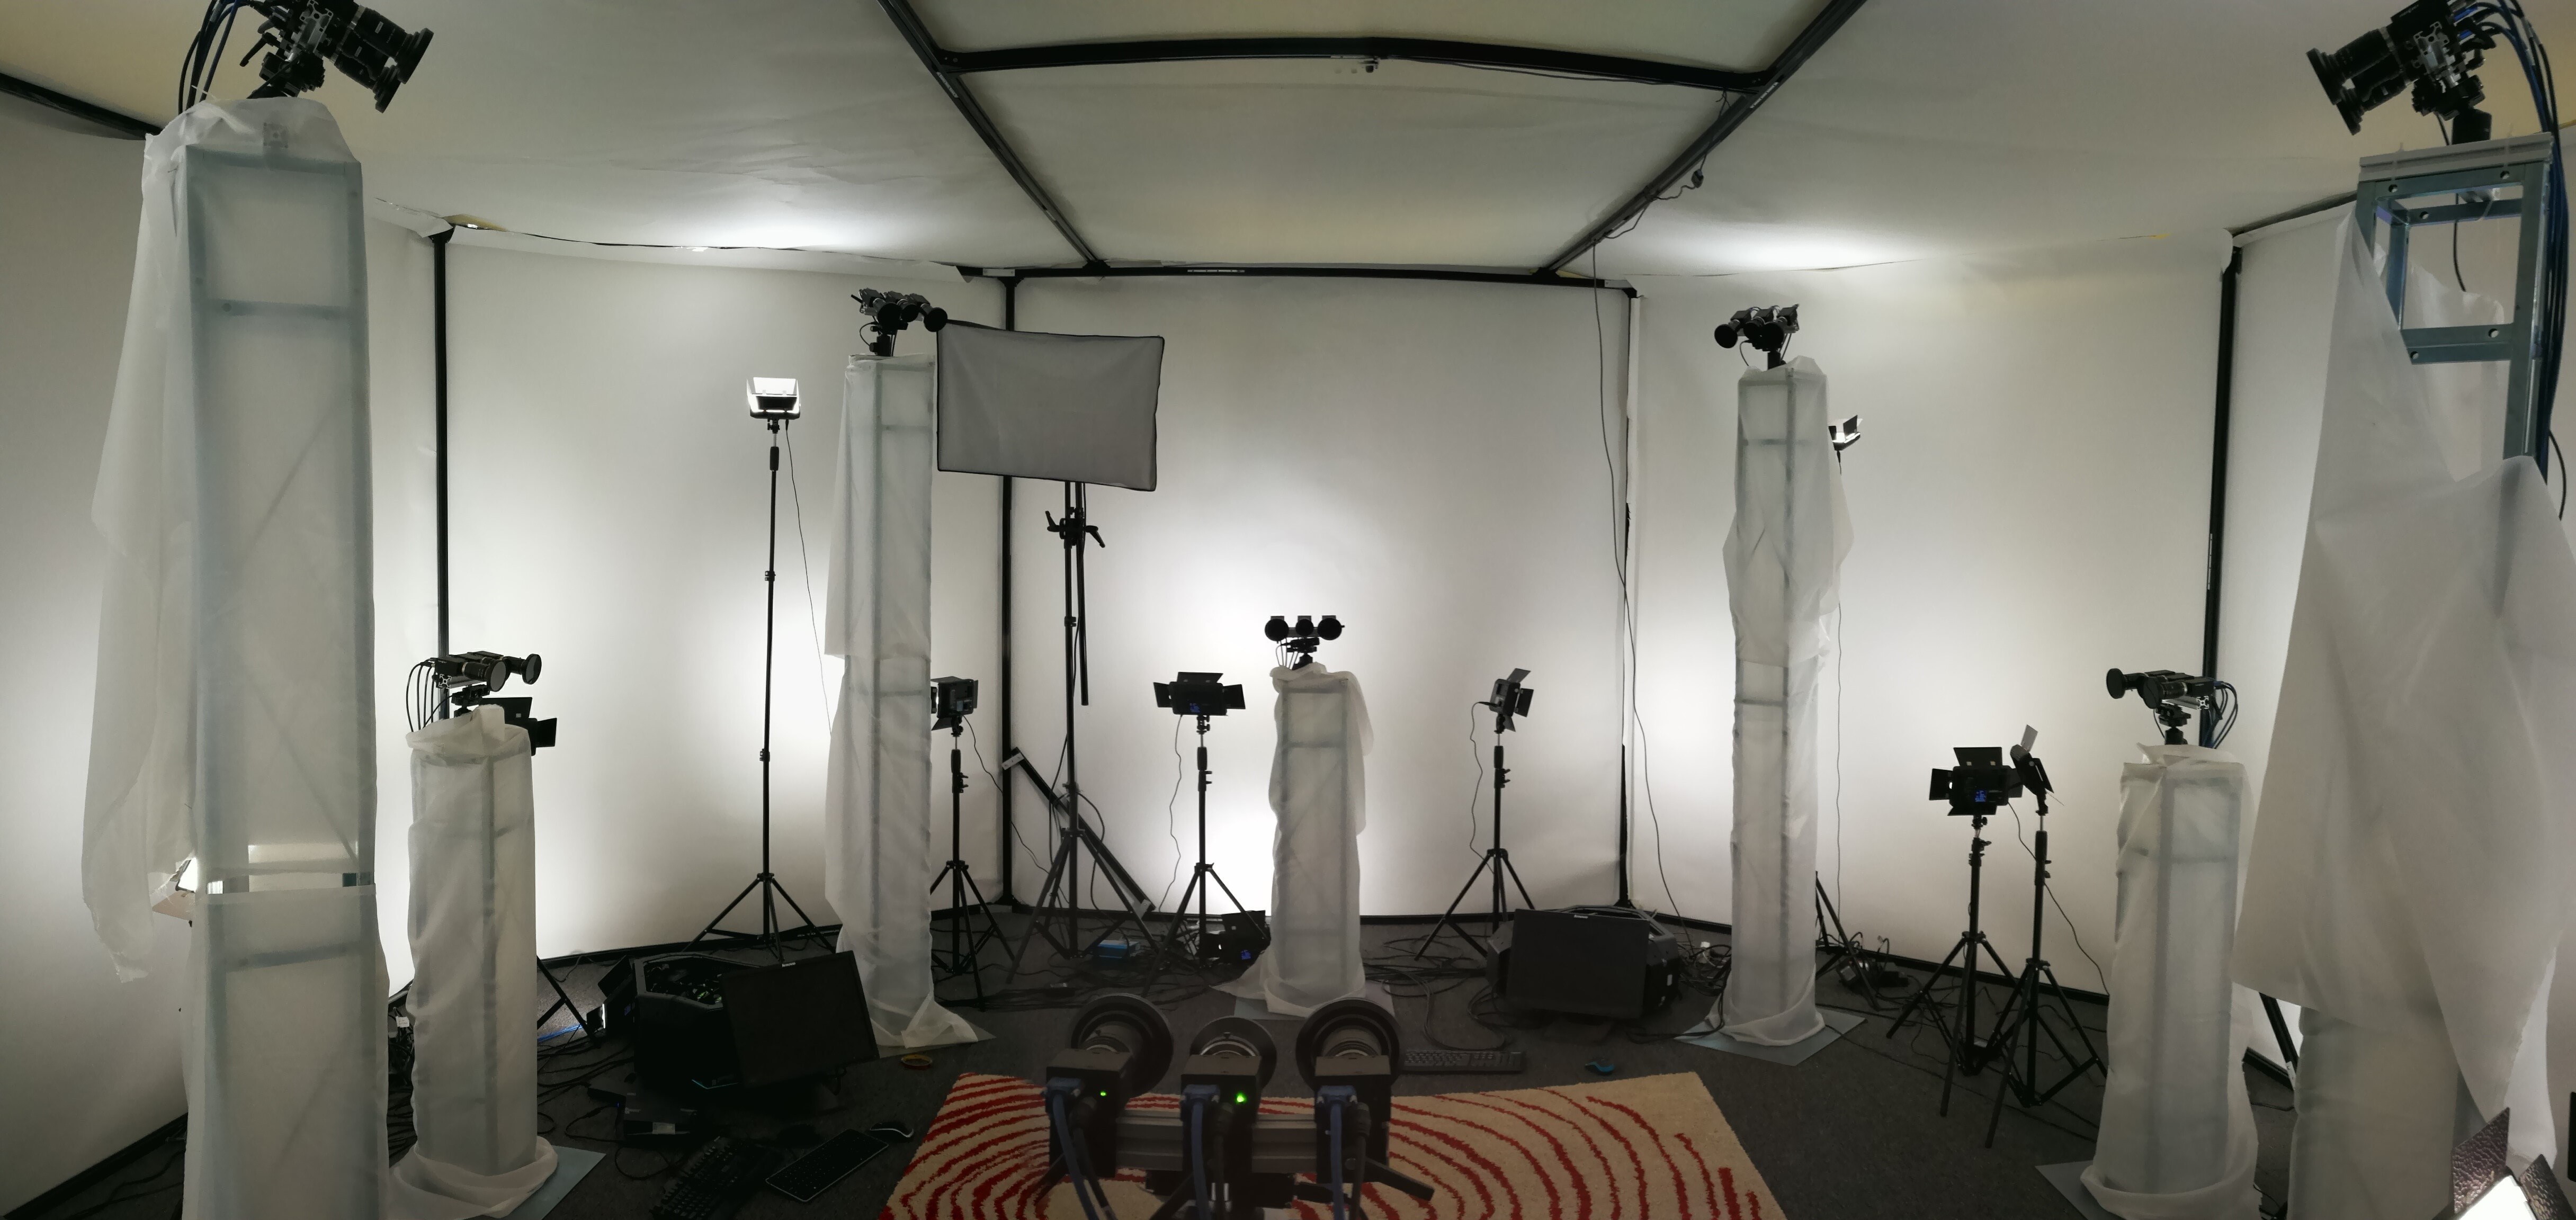
\includegraphics[scale=0.08]{image/rig.jpg}
\caption{Our multi-camera system with 8 camera pods pointing inwards.}
\label{fig:rig}
\end{figure*}

We employ 8 camera pods around the working space looking inwards for a full capture as shown in Figure~\ref{fig:rig}. Each pod consists of a color camera and 2 Near Infra-Red cameras (NIR). A laser pointer is used to produce special patterns, with it depth images can be achieved by the 2 NIR cameras using depth estimation methods.


\subsection{Camera model}
Let $\mathbf{P}$ be the 3D space coordinates of a point $\emph{P}$, and $\mathbf{p}$ the 2D coordinates of its projection in the image plane, the model of a pin-hole camera is usually described as
\begin{equation}
z_{p}\mathbf{p}=\mathbf{K_{in}}\mathbf{K_{ex}}\mathbf{P},
\end{equation}
where $z_{p}$ is the projective depth of point $\emph{P}$, $\mathbf{K_{in}}$ and $\mathbf{K_{ex}}$ are the intrinsic and extrinsic parameters of the camera.
\subsection{Initial calibration}
The $\mathbf{K_{in}}$ and initial $\mathbf{K_{ex}}$ of each camera are calibrated by Kalibr~\cite{Maye2013Self} pairwisely because of the lack of the common overlapping fields of view, including the 8 color cameras' extrinsic parameters $\{\mathbf{K_{ex}}_{i}\}_{i=1,...,8}$. The extrinsic parameters from the 2 NIR cameras to the color camera in the same camera pod are also achieved, but these extrinsic parameters are fixed and used to estimate the depth in each view.

\subsection{Global optimization}

We use a $6\times7$ checkerboard with squares of 117 mm for the optimization. The user is requested to move the checkerboard in front of the cameras freely in the working space. The checkerboard can be simultaneously seen in three or four views usually. Then the 42 corners on the checkerboard can be detected in each group. We can estimate the 3D space coordinates $\mathbf{P_{c}}$ of each corner from the corresponding 2D coordinates $\{\mathbf{p_{c}}_{j}\}_{j=1,...,n}$ by triangulation, where $n$ is the number of the views that the checkerboard can be seen in at the same time. To make the optimization result be more consistent to the whole system, we also use the images with checkerboard on the ground which allows the checkerboard corners can be seen in all the 8 cameras,  as shown in Figure~\ref{fig:checkerboard}. This will help to reduce the accumulative error and inconsistence caused by the pairwise calibration. The aim of the optimization is to minimize the sum of all reprojection errors with respect to all 3D points and extrinsic parameters, which is described as
\begin{equation}
E(\{\mathbf{K_{ex}}_{i}\})=\sum_{i}\sum_{j}((\mathbf{K_{in}}_{i}\mathbf{K_{ex}}_{i}\mathbf{P_{c}}_{j})-\mathbf{p_{c}}_{ij})^{2}.
\end{equation}

We use an open source software package called sba to solve this problem~\cite{lour09}.


\begin{figure}[ht]
%
\begin{minipage}[b]{.48\linewidth}
  \centering
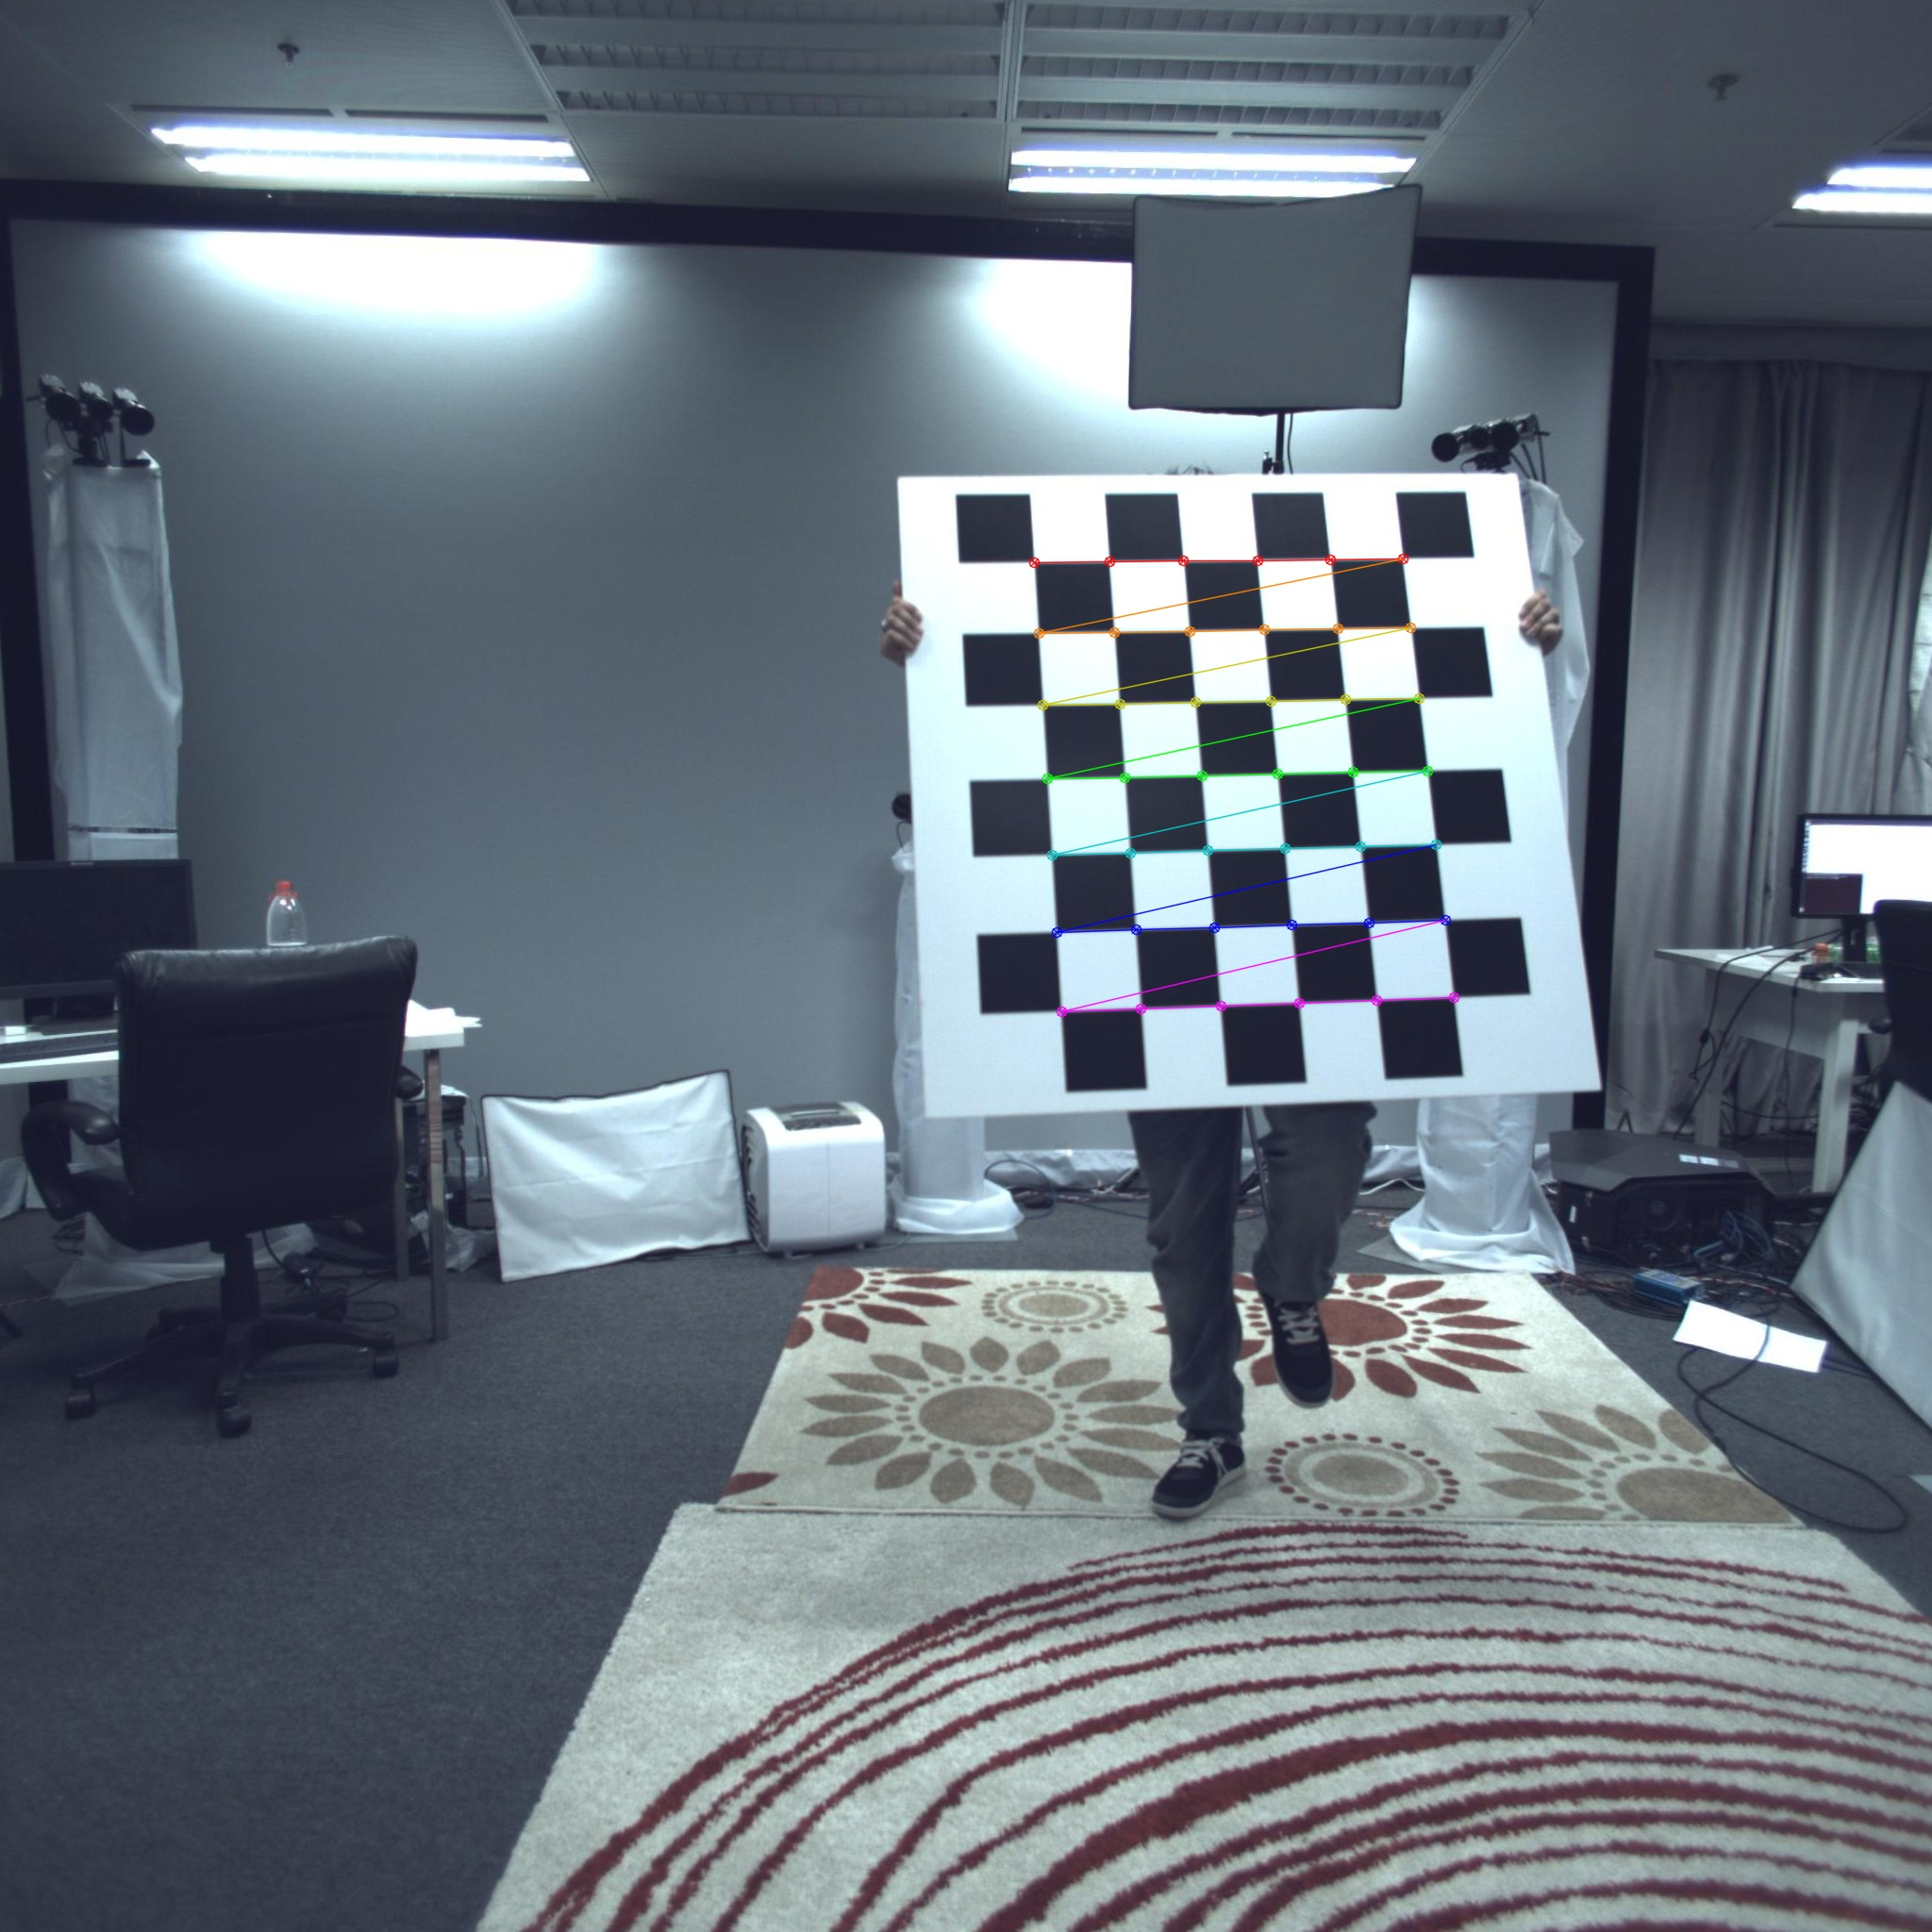
\includegraphics[scale=0.058]{image/free.jpg}
  \vspace{0cm}
  \centerline{(a)}\medskip
\end{minipage}
\hfill
\begin{minipage}[b]{0.48\linewidth}
  \centering
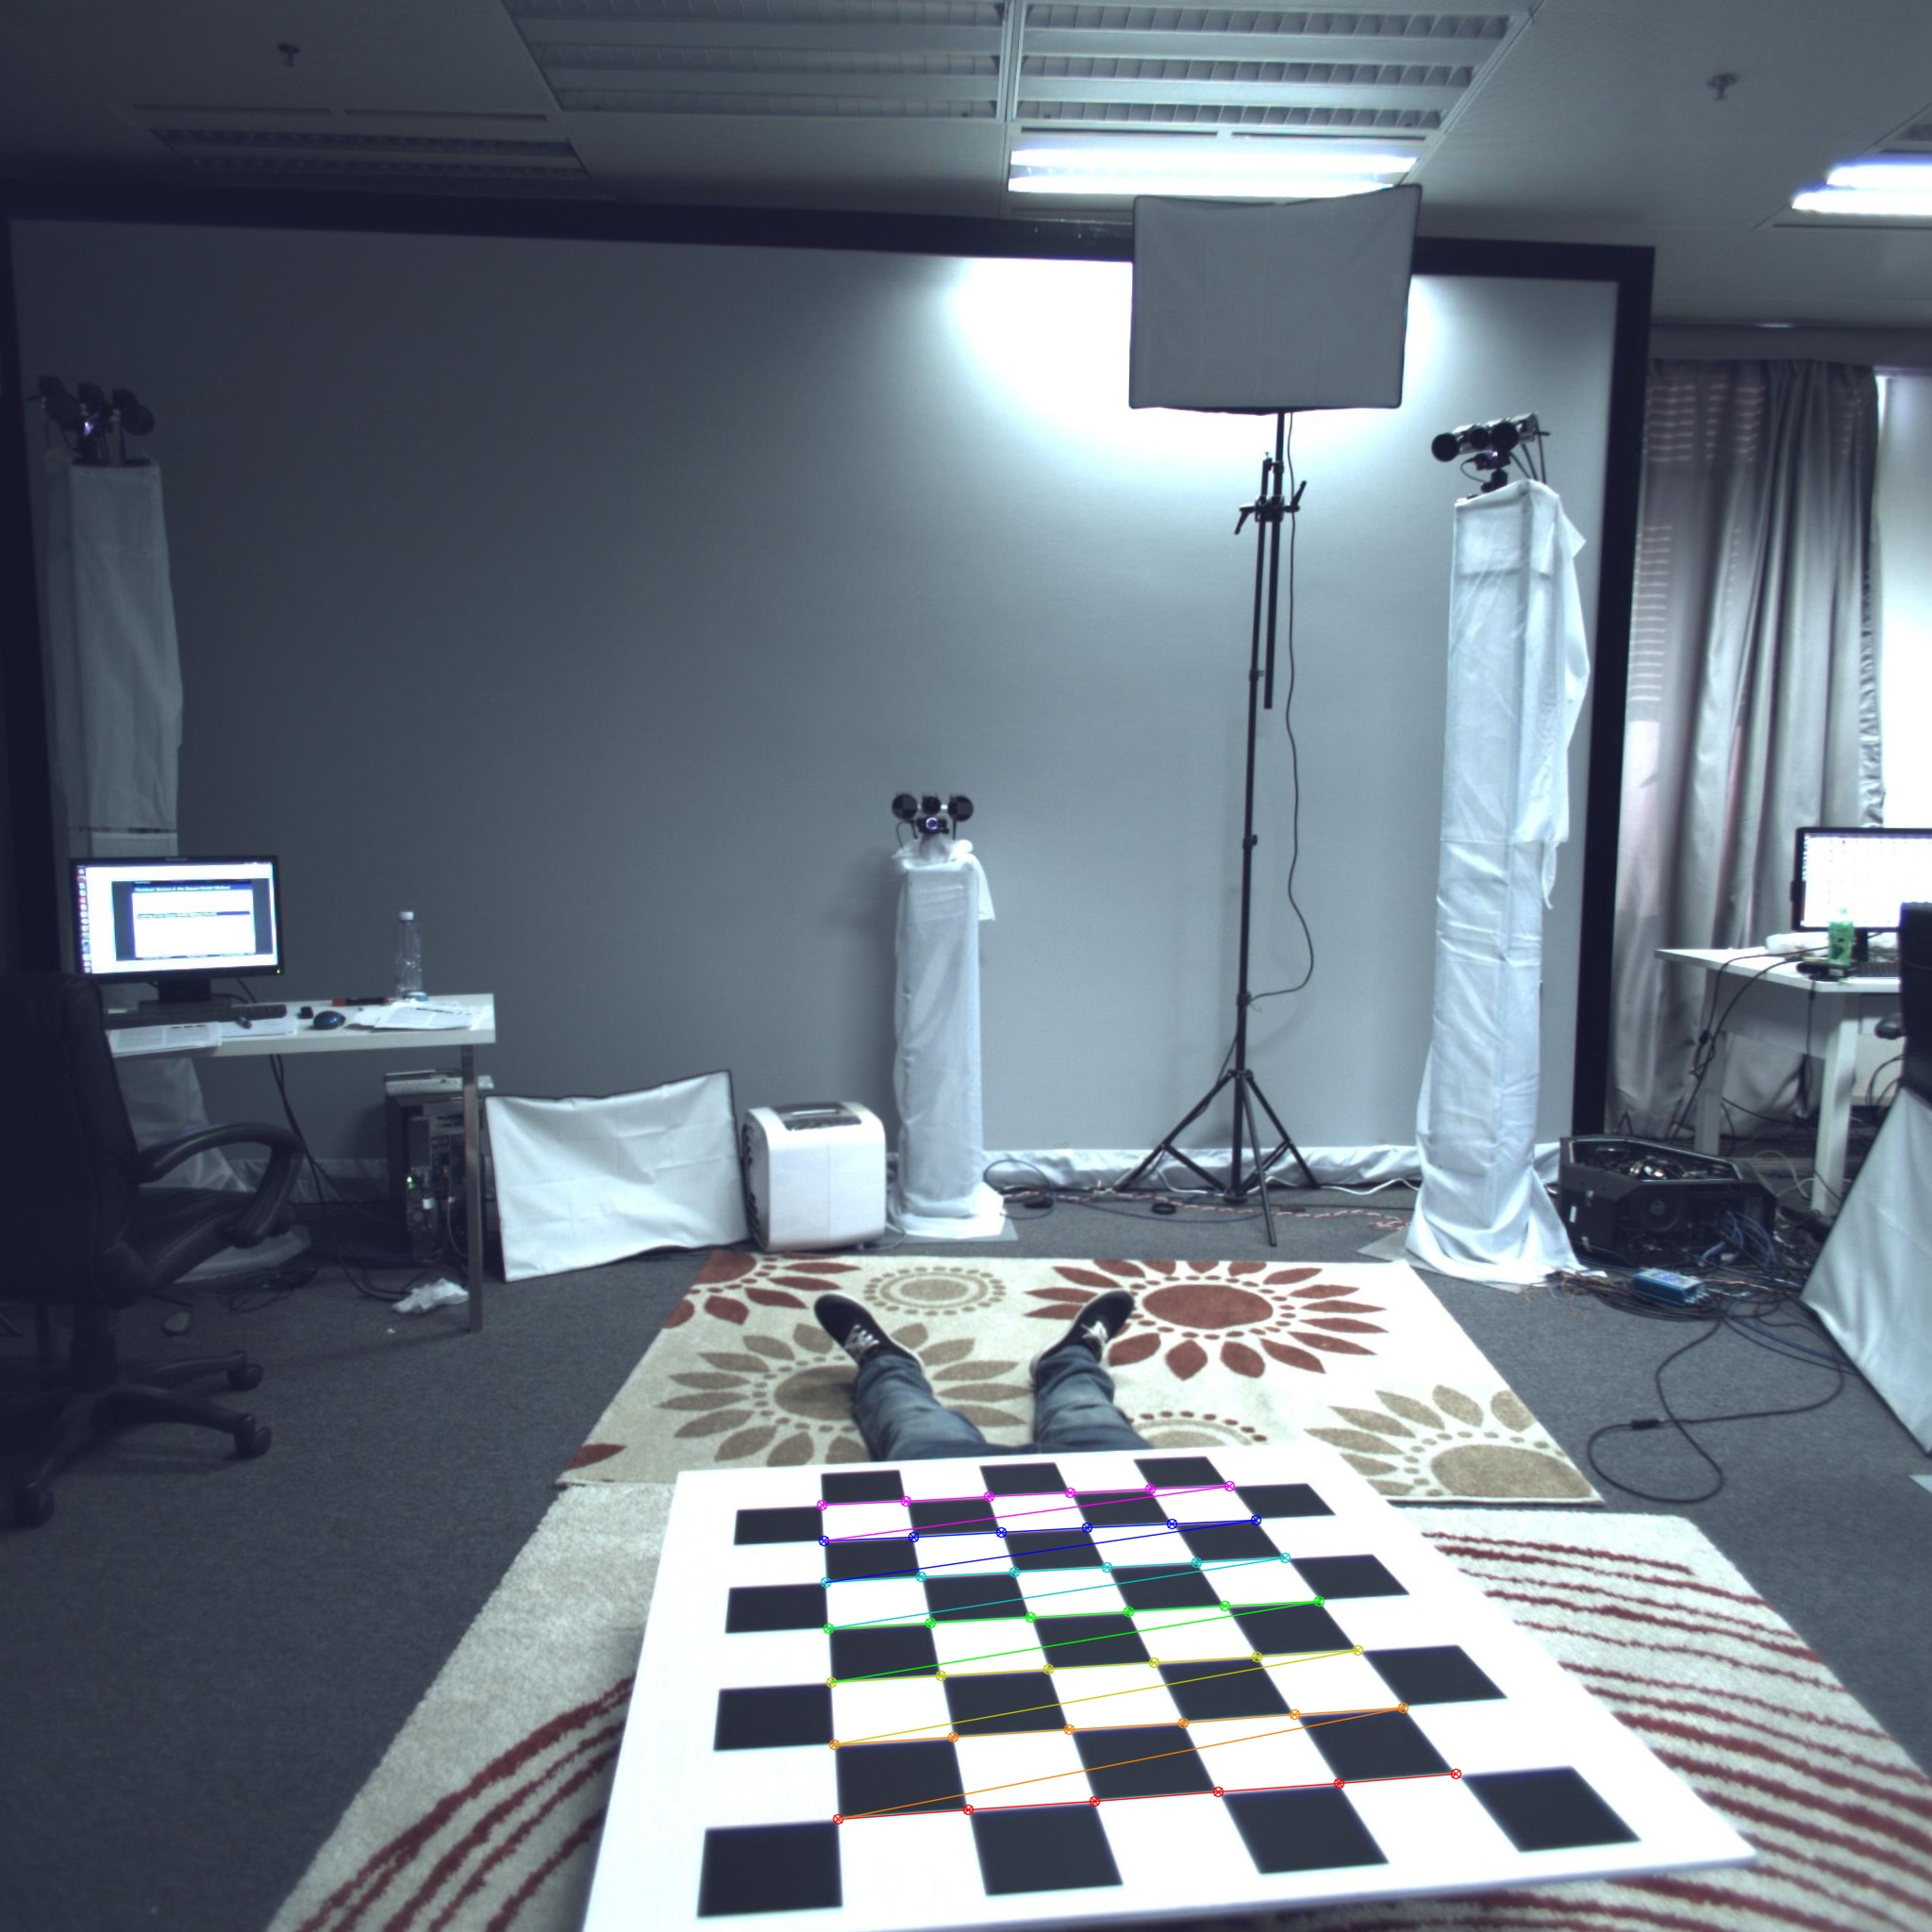
\includegraphics[scale=0.058]{image/ground.jpg}
  \vspace{0cm}
  \centerline{(b)}\medskip
\end{minipage}
%
\caption{Results of the checkerboard corners detection. (a): Results when the user moves freely. (b): Results when the checkerboard is on the ground. }
\label{fig:checkerboard}
\end{figure}
\section{point cloud registration}

We achieve the depth data from the 2 NIR cameras using depth estimation methods~\cite{Bleyer2011PatchMatch}. Although after the global optimization, we can get a result with less reprojection error, but it may not be the optimal solution to the 3D reconstruction beacause the quality of depth estimation also influence the final result. If the depth and camera parameters are both accurate enough, the point clouds of different views should align very well. However, the error cannot be avoided completely.

We reconstruct the point cloud of one view using the depth data, found the distortion on the boundary of the model, especially near the head, as shown in Figure~\ref{fig:deptherror}. Moreover, although the reprojection error after the global optimization mentioned in the last section is at sub-pixel level, we also find the separation between the point cloud of different views, effecting the quality of reconstruction. To minimize the error from depth data and achieve high-quality reconsturction results, we use ICP to map the inaccurate depth to a 3D model by point cloud registration.
\begin{figure}[ht]
\centering
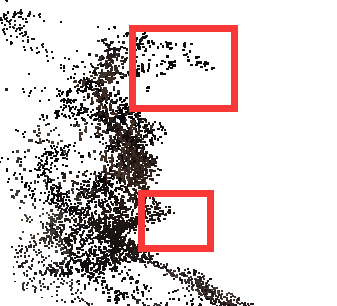
\includegraphics[scale=0.4]{image/depth_error.png}
\caption{The distortion near the head of the model of a single view which is caused by the inaccurate depth estimation.}
\label{fig:deptherror}
\end{figure}
For each point reconstructed by the depth image, we consider an estimation
\begin{equation}
\mathbf{\tilde{P}}_{ij}=f_{i}(\mathbf{P}_{j}),
\end{equation}
where $\mathbf{P}_{j}$ is the true 3D coordinates in the camera coordinate system. $f_{i}$ is a nonlinear function for view $i$, represent the depth influence. $\mathbf{\tilde{P}}_{ij}$ is the 3D coordinates we get from the depth data and intrinsic parameters in view $i$. With the extrinsic parameter, we can transform all the points into the world coordinate system. The estimation can be written as
\begin{equation}
\mathbf{\hat{P}}_{gj}=g(\mathbf{K_{ex}}_{i})f_{i}(\mathbf{P}_{j}),
\end{equation}
where $\mathbf{\hat{P}}_{gj}$ is the 3D coordinates in the world coordinate system we reconstruct from the depth and camera parameters. ICP can be replaced as a rigid transform to all views
\begin{equation}
\mathbf{\tilde{\hat{P}}}_{gj}=M_{i}g(\mathbf{K_{ex}}_{i})f_{i}(\mathbf{P}_{j})=g(\mathbf{K_{ex}}_{i})M_{i}f_{i}(\mathbf{P}_{j}),
\end{equation}
where $\mathbf{\tilde{\hat{P}}}_{gj}$ is the coordinates of the point after the alignment. The transform $M_{i}$ can refine the error caused by $f_{i}$, and improve the quality of the result of 3D reconstruction.

We choose the point cloud of view 1 as the reference, align the point cloud of view 2 to it, combine the result of the two views, then align the point cloud of view 3 to the combined result and so on. Each ICP process produce a transformation matrix, then we can map the inaccurate depth to a high-quality 3D model using the rigid transformation.




% References should be produced using the bibtex program from suitable
% BiBTeX files (here: strings, refs, manuals). The IEEEbib.bst bibliography
% style file from IEEE produces unsorted bibliography list.
% -------------------------------------------------------------------------
\bibliographystyle{IEEEbib}
\bibliography{icme2018template}

\end{document}
